\section{The basics of Quantum Monte-Carlo}

% \begin{frame}
%  \frametitle{Unfamiliar with Quantum Mechanics?}
%  
%  Imagine states as vectors and operators as matrices:
%  
%  \begin{align*}
%   \ket{\Psi} &\to \left(\begin{array}{c} a\\ b \end{array}\right). \\
%   &\\
%   \bra{\Psi} &\to \left(a^\ast,\, b^\ast\right). \\
%   &\\
%   \OP{H} &\to \left(\begin{array}{cc} h_{11} & h_{12} \\ h_{21} & h_{22} \end{array}\right).                         
%  \end{align*}
%  
%  \pause
%  Ground state energy: Lowest eigenvalue of $\OP{H}$.
%  \pause
%  
%  Ground state: Corresponding eigenvector $\ket{\Psi_0}$.
%  
%  \end{frame}

 

\subsection{The basic idea}

\begin{frame}

\frametitle{The basic idea}

\begin{itemize}
  \item Project an arbitrary state down on the exact ground state.
  \item Model this state by an ensemble of random walkers.
  \item Simulate the projection using stochastic processes.
\end{itemize}

\end{frame}

% \subsection{The projection}

\begin{frame}
\frametitle{The projection}
%  Applying the \textit{projection operator} $\OP{P}(\tau)$ on an arbitrary state $\ket{\Psi_T}$ projects the state onto the ground state of $\OP{H}$ as $\tau\to\infty$.  
%  \pause
%   \begin{align*}
%    \onslide<2->{\OP{P}(\tau)\ket{\Psi_T} &= \exp(-(\OP{H} - E_0)\tau)\ket{\Psi_T} \\}
%    \onslide<3->{&= \exp(-(\OP{H} - E_0)\tau)\sum_{k} C_k\ket{\Psi_k} \\}
%    \onslide<4->{&= \sum_{k} C_k\exp(-(E_k - E_0)\tau) \ket{\Psi_k} \\}
%    \onslide<5->{&= C_0\ket{\Psi_0} + \sum_{k=1} C_k\exp(-\Delta E_k\tau) \ket{\Psi_k},}
%   \end{align*}
  \begin{align*}
  \OP{P}(\tau) &= \exp(-(\OP{H} - E_0)\tau) \\
  \OP{P}(\tau)\ket{\Psi_T} &= C_0\ket{\Psi_0} + \sum_{k=1} C_k\exp(-\Delta E_k\tau) \ket{\Psi_k}
  \end{align*}

  where $\Delta E_k > 0$ and $C_k = \braket{\Psi_k}{\Psi_T}$. 
  
  \pause 
  
   In other words
 
 \begin{equation*}
  \lim_{\tau\to\infty}\bra{\mathbf{r}}\OP{P}(\tau)\ket{\Psi_T} = \braket{\Psi_0}{\Psi_T}\Psi_0(\mathbf{r}).
 \end{equation*}

\end{frame}

\begin{frame}
 \frametitle{The stochastic process}
 In order to relate the projection process to a \textit{Markov chain} Monte-Carlo process, $\tau$ needs to be split into sequential steps $\delta\tau$. 
 \shift
 
Using that 
 
%  \begin{align*}
%   \OP{P}(\tau + \delta\tau) &= \exp(-(\OP{H} - E_T(\tau + \delta\tau))(\tau + \delta\tau)) \\
%                             &=  \exp(-(\OP{H} - E_T(\tau + \delta\tau))\delta\tau) \\
%                             & \qquad \times\exp(-(\OP{H} - E_T(\tau + \delta\tau))\tau) \\
%                            \onslide<3->{ &\simeq \exp(-(\OP{H} - E_T(\tau + \delta\tau))\delta\tau)\OP{P}(\tau),}
%  \end{align*}

\begin{equation*}
 \OP{P}(\tau + \delta\tau) = \exp(-(\OP{H} - E_0)\delta\tau)\OP{P}(\tau),
\end{equation*}

yields 


\begin{align*}
\Phi(\mathbf{r}, \tau + \delta\tau) &\equiv \bra{\mathbf{r}}\OP{P}(\tau + \delta\tau)\ket{\Psi_T} \\
   &= \int_\mathbf{r'}\bra{\mathbf{r}}\exp(-(\OP{H} - E_0)\delta\tau)\ket{\mathbf{r'}}\Phi(\mathbf{r'}, \tau)\mathrm{d}\mathbf{r'},
\end{align*}

\pause

\begin{equation*} 
\bra{\mathbf{r}}\exp(-(\OP{H} - E_0)\delta\tau)\ket{\mathbf{r'}} \equiv G(\mathbf{r'}, \mathbf{r}; \delta\tau).
\end{equation*}


% \onslide<3->{where the relation is approximate due to $E_T$ not being constant.}
 
 
 
\end{frame}





% \begin{frame}
%   Let $\ket{\Phi(\tau)}$ represent $\OP{P}(\tau)\ket{\Psi_T}$. Using the relation from the previous slide reveals
%   \pause
%   \begin{align*}
%    \onslide<2->{\Phi(\mathbf{r}, \tau + \delta\tau) &= \braket{\mathbf{r}}{\Phi(\tau + \delta\tau)} \\ &= \bra{\mathbf{r}}\OP{P}(\tau + \delta\tau)\ket{\Psi_T} \\}
%    \onslide<3->{&\simeq  \bra{\mathbf{r}}\exp(-(\OP{H} - E_T)\delta\tau)\OP{P}(\tau)\ket{\Psi_T} \\}
%    \onslide<4->{&=\bra{\mathbf{r}}\exp(-(\OP{H} - E_T)\delta\tau)\ket{\Phi(\tau)}  \\}
%    \onslide<5->{&= \int_\mathbf{r'}\bra{\mathbf{r}}\exp(-(\OP{H} - E_T)\delta\tau)\ket{\mathbf{r'}}\Phi(\mathbf{r'}, \tau)\mathrm{d}\mathbf{r'},}
%   \end{align*}
%   
%   \pause\pause\pause\pause
%   where $\bra{\mathbf{r}}\exp(-(\OP{H} - E_T)\delta\tau)\ket{\mathbf{r'}} \equiv G(\mathbf{r'}, \mathbf{r}; \delta\tau)$ is a \textit{Green's function} interpreted as the transition probability between $\mathbf{r}$ and $\mathbf{r'}$.
%     
% \end{frame}

\begin{frame}
\frametitle{The stochastic process}
 In order to relate the Green's function to well known Markov processes, the exponential is split
 
 \begin{align*}
  \exp(-(\OP{H} - E_0)\delta\tau) &= \exp\left(\frac{1}{2}\nabla^2\delta\tau - (\OP{V} - E_0)\delta\tau\right)\\
     &= \exp\left(\frac{1}{2}\nabla^2\delta\tau\right)\exp( - (\OP{V} - E_0)\delta\tau) \\
     & \qquad  + \mathcal{O}(\delta\tau^2),
 \end{align*}
 
which reads \textit{diffusion} and \textit{weighting}.
 
\end{frame}

\begin{frame}
%  In other words
%  
%  \begin{equation}
%   \lim_{\tau\to\infty}\bra{\mathbf{r}}\OP{P}(\tau)\ket{\Psi_T} = \braket{\Psi_0}{\Psi_T}\Psi_0(\mathbf{r}).
%  \end{equation}
% 
%  \pause
%  \textbf{Idea}: Use an arbitrary \textit{trial wave function} $\Psi_T(\mathbf{r})$ and perform the projection.
%  \shift
 
 \textbf{Problem}: Requires a priori knowledge of the exact ground state energy $E_0$.
 \shift
 
 \textbf{Solution}: Introduce a \textit{trial energy} $E_T(\tau)$ instead of $E_0$ in the Green's function.
 
\end{frame}

\begin{frame}
 \textbf{Problem}: The Green's function has singular points in the Coulomb interaction.
 \shift
 
 \textbf{Solution}: By evolving $f(\mathbf{r}, \tau) = \Phi(\mathbf{r}, \tau)\Psi_T(\mathbf{r})$ instead of $\Phi(\mathbf{r}, \tau)$ alone, the singularities are \emph{implicitly} taken care of.
  
 \end{frame}

 \begin{frame}
   Originally $\Phi(\mathbf{r}, \tau) = \bra{\mathbf{r}}\OP{P}(\tau)\ket{\Psi_T}$ solves:
 \begin{equation*}
  \frac{\partial \Phi(\mathbf{r}, \tau)}{\partial\tau} = \left[\frac{1}{2}\nabla^2 - \left(\OP{V} - E_T\right)\right]\Phi(\mathbf{r}, \tau).
 \end{equation*}
 
 \pause
 
 \textit{Importance sampled}:
  \begin{equation*}
  \frac{\partial f(\mathbf{r}, \tau)}{\partial\tau} = \left[\frac{1}{2}\nabla\cdot\left(\nabla - \mathbf{F}(\mathbf{r})\right) - (E_L(\mathbf{r}) - E_T)\right]f(\mathbf{r}, \tau),
 \end{equation*}
 
 where
 
\begin{equation*}
  \mathbf{F}(\mathbf{r}) =  2\Psi_T(\mathbf{r})^{-1}\nabla \Psi_T(\mathbf{r})
\end{equation*}

is the \textit{quantum force} and 

\begin{equation*} 
E_L(\mathbf{r}) = \Psi_T(\mathbf{r})^{-1}\OP{H}\Psi_T(\mathbf{r})
\end{equation*}

is the \textit{local energy}. 

\end{frame}

\begin{frame}
 The Green's functions have closed form solutions on the form
 
 \begin{align*}
  G_{\mathrm{Diff}}(\mathbf{r}', \mathbf{r}; \delta\tau) &\propto \exp\left(-\left|\mathbf{r}-\mathbf{r}' - D\delta\tau \mathbf{F}(\mathbf{r})\right|^2/4D\delta\tau\right), \\
  G_{\mathrm{W}}(\mathbf{r}', \mathbf{r}; \delta\tau) &\propto \exp\left(-\left(\frac{1}{2}\left[E_L(\mathbf{r}) + E_L(\mathbf{r}')\right] - E_T\right)\delta\tau\right),
 \end{align*}

 where $\mathrm{W}$ denotes \textit{weighting}.
 \shift
 
 $\Psi_T(\mathbf{r})$ is tailored to cancel singularities in $E_L(\mathbf{r})$. 
 
 
\end{frame}

% \begin{frame}
%  The local energy dependence in the branching Green's function implicitly takes care of the singularities in $\OP{V}$. 
%  \shift
%  
%  This is done by introducing the \textit{Jastrow factor} in $\Psi_T(\mathbf{r})$
%  
%  \begin{equation}
%   J(\mathbf{r}) = \prod_{i > j}^N \exp\left(a_{ij} \frac{r_{ij}}{1 + \beta r_{ij}}\right),
%  \end{equation}
%  
%  where $r_{ij} = |\mathbf{r}_i - \mathbf{r}_j|$, $N$ is the number of particles, $\beta$ is a variational parameter, and $a_{ij}$ is a constant depending on the spin eigenvalues of particles $i$ and $j$.
%  \shift
%  
%  The Jastrow factor is tailored to cancel the singularities in the electron-electron Coulomb interaction as the relative distances decrease.
%  
% \end{frame}


\begin{frame}

 \frametitle{The Markov process}

%  \textbf{Idea}: The process of projection is modelled by letting an ensemble of walkers span $f(\mathbf{r}, \tau)$. An iteration involves diffusing all the walkers and distributing new weights. 
%  \shift
 
 \textbf{Problem}: The distribution $f(\mathbf{r}, \tau) = \Phi(\mathbf{r}, \tau)\Psi_T(\mathbf{r})$ is not exclusively positive unless the nodes (zeros) of $\Psi_T(\mathbf{r})$ matches those of $\Phi(\mathbf{r}, \tau)$. 
 \shift
 
 \textbf{Solution}: \emph{Fixing} the nodes of $f(\mathbf{r}, \tau)$ to match those of $\Psi_T(\mathbf{r})$ (the \textit{fixed node approximation}).
 
\end{frame}

\begin{frame}
\begin{figure}
 \begin{center}
  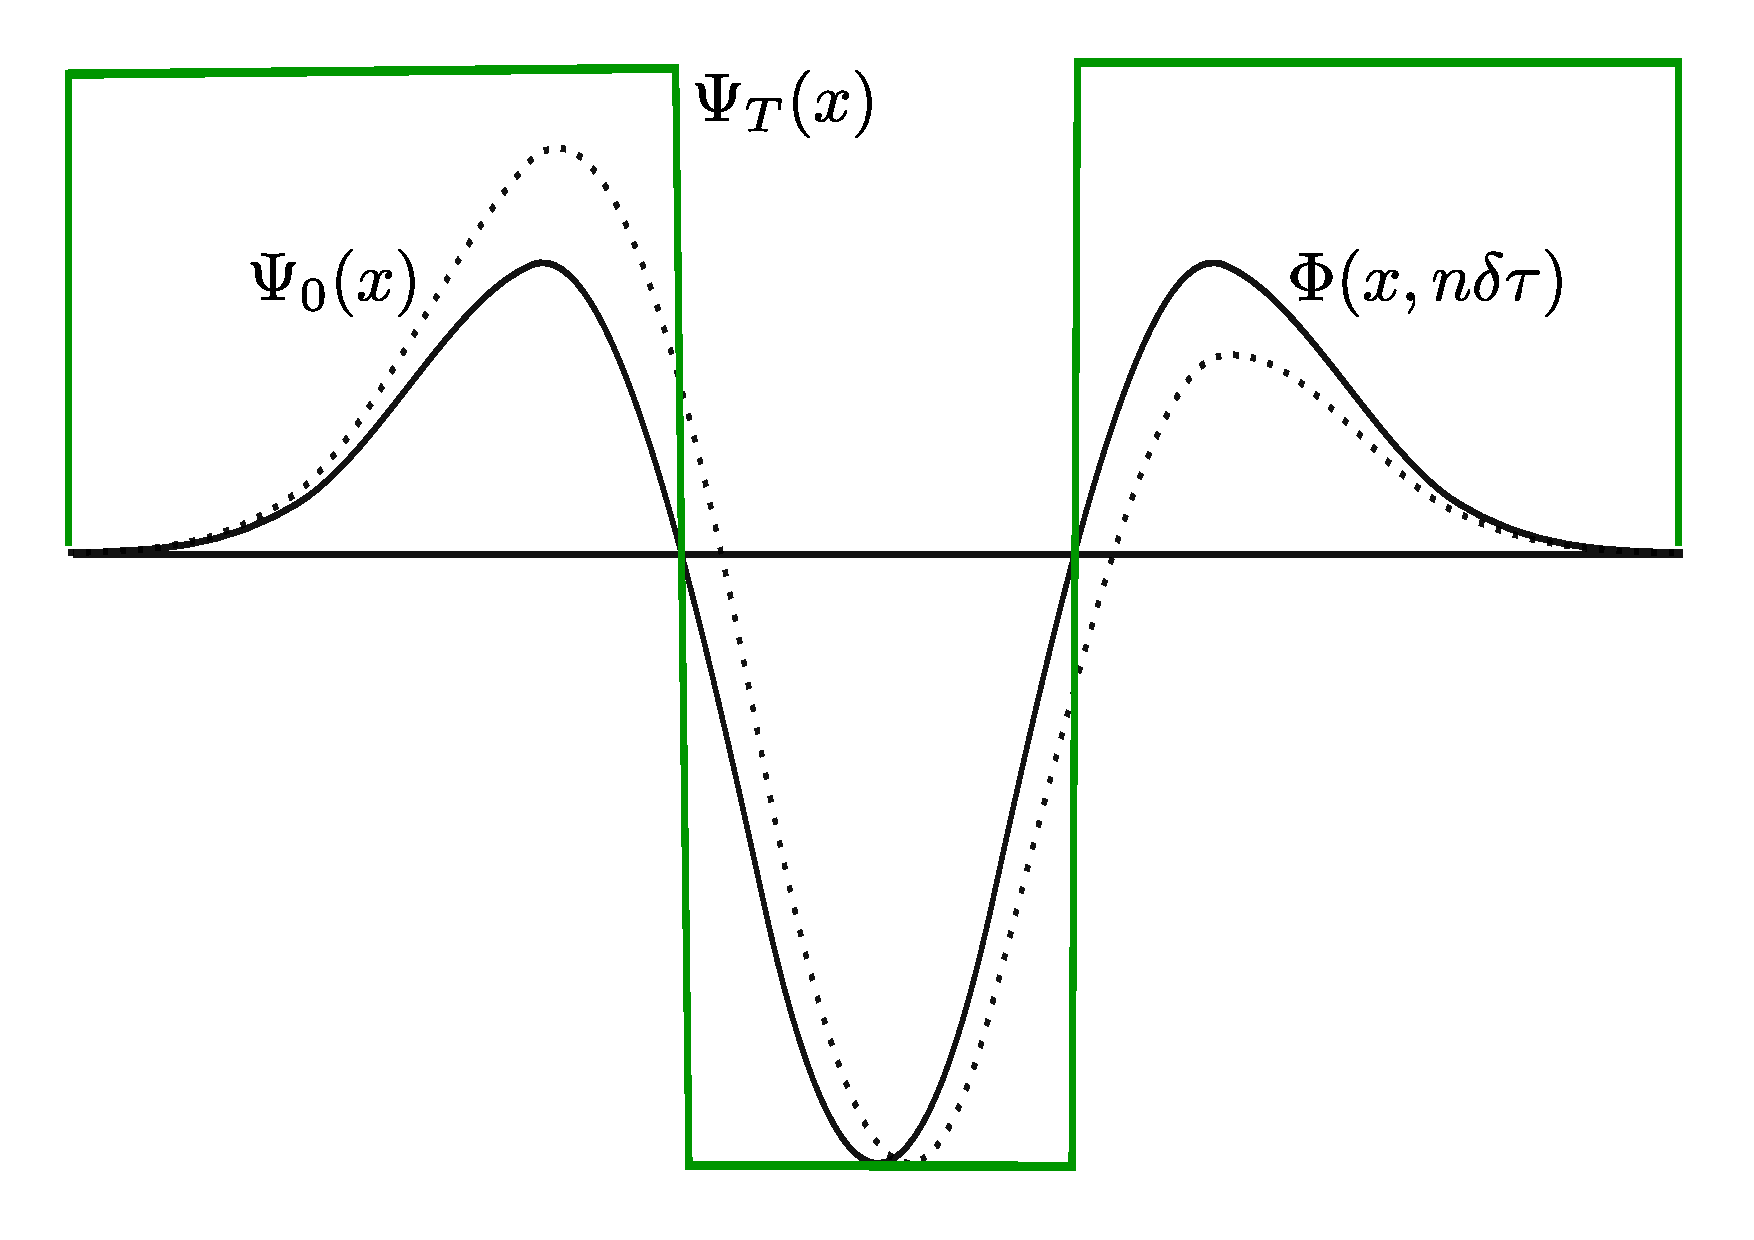
\includegraphics[scale=0.3]{../graphics/fixxednode.pdf}
 \end{center}
 \caption{The fixed node approximation illustrated. The nodes of $\Phi(x, n\delta\tau)$ is fixed to match those of $\Psi_T(x)$.}
\end{figure}
\end{frame}


\begin{frame}
\frametitle{Branching}

\textbf{Idea}: The weights are modelled by spawning and killing walkers with a rate equal to $G_\mathrm{W}$. 
\shift

\textbf{Problem}: $G_\mathrm{W}$ is not necessarily an integer.
\shift

\textbf{Solution}: The walker branch $\mathrm{floor}(G_\mathrm{B})$ times with a chance of one additional copy.


\vspace{0.5cm}
If zero branches, the walker is removed.

% \shift
% 
% Or more compact: Create 
% 
% \begin{equation}
% \overline{G}_\mathrm{B} = \mathrm{floor}(G_\mathrm{B} + a)
% \end{equation}
% 
% copies, where $a \in [0,\,1)$ is a uniformly distributed random number. If the value is zero, the walker dies.

\end{frame}


\begin{frame}
\frametitle{Branching}

\begin{figure}
\begin{center}
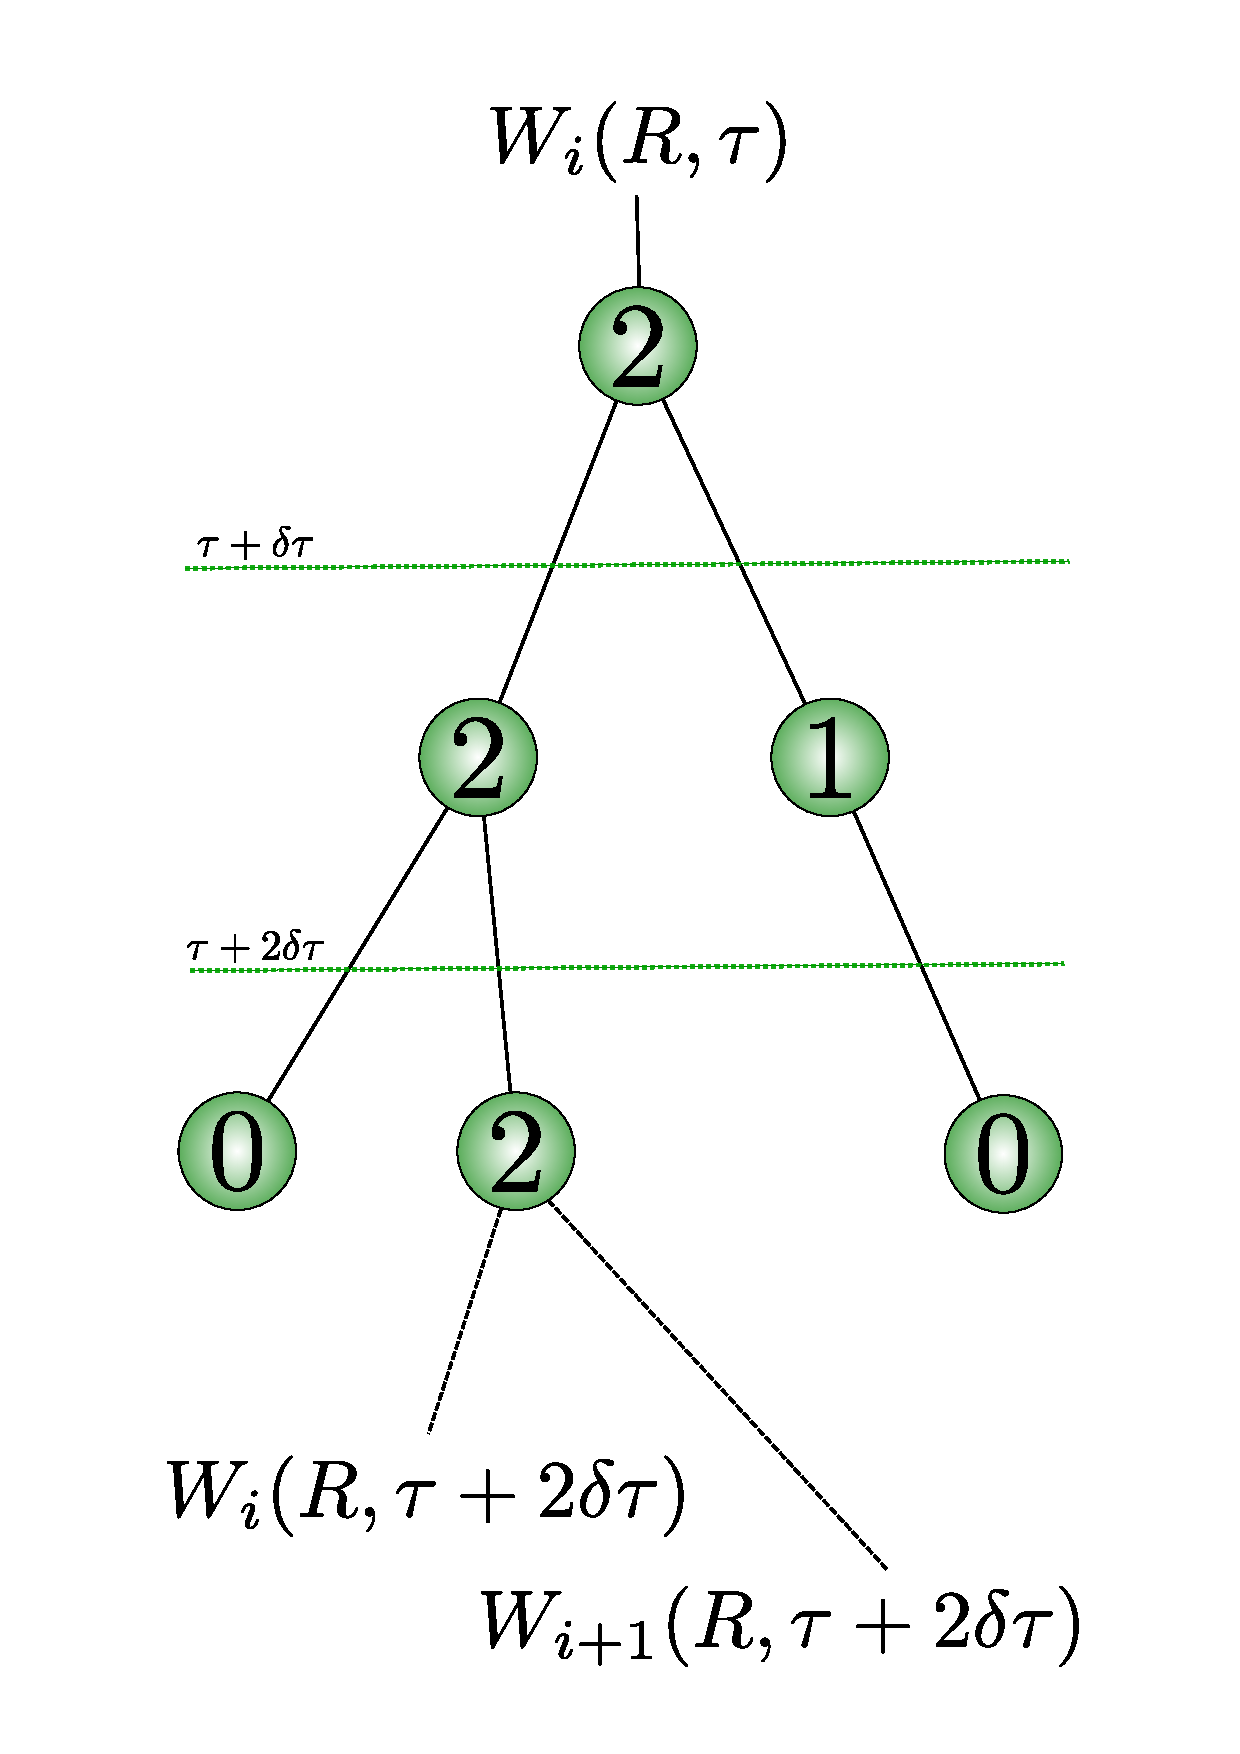
\includegraphics[scale=0.2]{../graphics/branching.pdf}
\end{center}
\caption{Branching illustrated. The integer values represent $\overline{G}_\mathrm{B}$.}
\end{figure}

\end{frame}

\begin{frame}
 \frametitle{Diffusion}
 
%  The diffusion equation representing $G_\mathrm{Diff}$ is the so-called \textit{Fokker-Planck equation}. 
%  \shift
%  
%  Anisotropic diffusion process. The quantum force pushes the walkers into regions of higher probability. 
%  \shift
%  
%  According to the Fokker-Planck formalism, 

According to the introduced diffusion process, the new position $\mathbf{r}_{i+1}$ is calculated from the old one, $\mathbf{r}_i$, as follows
 
 \begin{equation*}
  \mathbf{r}_{i+1} = \mathbf{r}_i + D\delta\tau\mathbf{F}(\mathbf{r}_i) + \mathbf{\xi}, 
 \end{equation*}

where $\mathbf{\xi}$ is a vector of normal distributed random numbers with variance $\sqrt{2D\delta\tau}$.
 
\end{frame}

\begin{frame}
\frametitle{Diffusion}

\textbf{Problem}: Due to a finite time step, the previous equations do not guarantee convergence.  
\shift

\textbf{Solution}: The \textit{Metropolis algorithm} will correct this bias:  

\begin{equation*}
  A(i\,\rightarrow\,j) = \min\{R_G(i\,\rightarrow\,j)R_\psi(i\,\rightarrow\,j)^2, \,1\},
\end{equation*}

where $i\,\rightarrow\,j$ denotes a transition from state $i$ to state $j$, $A$ is the probability of accepting the transition, 

\begin{equation*}
 R_G(i\,\rightarrow\,j) = G_\mathrm{Diff}(\mathbf{r}_{j}, \mathbf{r}_{i}; \delta\tau)/G_\mathrm{Diff}(\mathbf{r}_{i}, \mathbf{r}_{j}; \delta\tau),
\end{equation*}

and

\begin{equation*}
 R_\psi(i\,\rightarrow\,j) = |\Psi_T(\mathbf{r}_j)/\Psi_T(\mathbf{r}_i)|.
\end{equation*}

\end{frame}


%% 15

\begin{frame}
 \frametitle{Recap}
 
 \begin{itemize}
 \item The distribution at any stage is given as the histogram of the walkers' configurations.
 \pause \item The projection process involves diffusing the walkers and calculating weights.
 \pause \item Efficient sampling by using the quantum force.
 \pause \item Unbiased sampling by using the Metropolis algorithm.
 \pause \item Transition from $|\Psi_T|^2 \to f(\mathbf{r}, \tau)$ by including the weights.
%  \pause \item The Metropolis algorithm corrects the bias introduced by a finite step length. Ensures that the walkers follow $|\Psi_T(\mathbf{r})|^2$.
%  \pause \item After each diffusion step, the walker is either killed or cloned based on the value of the branching Green's function. This ensures that the distribution of walkers follows $f(\mathbf{r}, \tau)$ and not $|\Psi_T(\mathbf{r})|^2$.
 \end{itemize}

\end{frame}

\subsection{Explicit methods}

\begin{frame}
 \frametitle{Variational Monte-Carlo}
 Neglecting the branching results in a method known as \textit{Variational Monte-Carlo} (VMC).
 \shift
 
 Corresponds to calculating $\bra{\Psi_T}\OP{H}\ket{\Psi_T}$ using a standard Monte-Carlo approach
 
 \begin{equation*}
  \bra{\Psi_T}\OP{H}\ket{\Psi_T} = \int_\mathbf{r} |\Psi_T(\mathbf{r})|^2 E_L(\mathbf{r})\mathrm{d}\mathbf{r} \simeq \frac{1}{N}\sum_{i=1}^N \frac{1}{\Psi_T(\mathbf{r_i})}\OP{H}\Psi_T(\mathbf{r}_i) 
 \end{equation*}
 
\end{frame}

\begin{frame}
 \frametitle{\textbf{Variational} Monte-Carlo}
 
 Variational Monte-Carlo will always result in an energy which is greater or equal to the exact ground state energy
 
 \begin{align*}
  \bra{\Psi_T}\OP{H}\ket{\Psi_T} &= \sum_{ij} C_i^\ast C_j \underbrace{\bra{\Psi_i} \OP{H} \ket{\Psi_j}}_{E_i\delta_{ij}} \\
                                 &= \sum_i |C_i|^2 E_i \\
                                 &= \sum_i |C_i|^2 (E_0 + \Delta E_i) \\
                                 &= E_0 \underbrace{\sum_i |C_i|^2}_{1} + \underbrace{\sum_i |C_i|^2\Delta E_i}_{\ge 0} \\
                                 &\ge E_0.
 \end{align*}
\end{frame}

\begin{frame}
 \frametitle{Limitations: VMC}
 
 VMC is extremely robust, however, extremely dependent on a good ansatz for $\Psi_T(\mathbf{r})$.
 
\end{frame}



\begin{frame}
 \frametitle{Limitations: VMC}
 
 \begin{figure}
  \begin{center}
   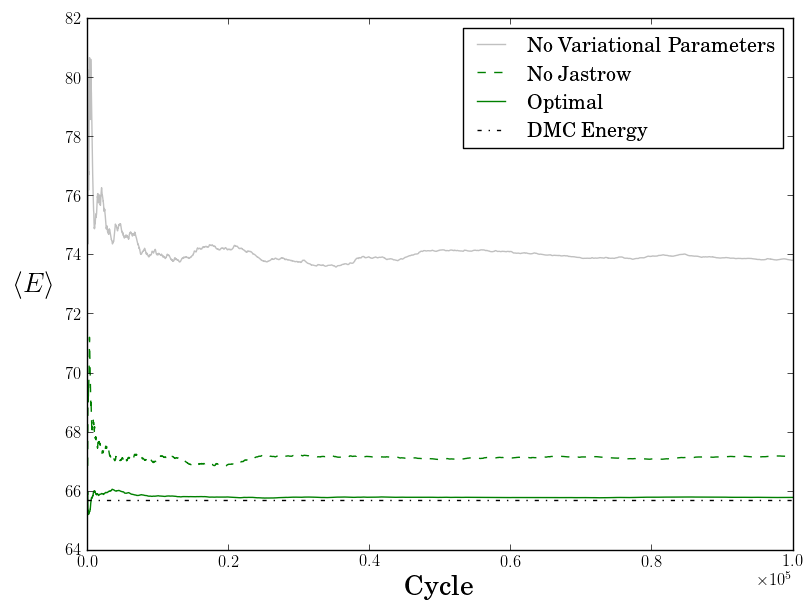
\includegraphics[scale=0.35]{../graphics/WFComp.png}
  \end{center}
  \caption{Comparison of different trial wave functions for a two-dimensional 12-particle quantum dot with unit frequency.}
 \end{figure}
 
\end{frame}

% \begin{frame}
%  The \textit{variational principle} introduced in the previous slide opens up the possibility to introduce \textit{variational parameters} in $\Psi_T(\mathbf{r})$ whose values are found by minimizing the VMC energy in the parameter space.
%  \shift
%  
%  Already have $\beta$ from the Jastrow factor. 
%  \shift
%  
%  The \textit{spatial} wave function is modelled as a single \textit{Slater determinant}, which can be split into two parts $|\mathbf{S(\mathbf{r})}^\uparrow|$ and $|\mathbf{S(\mathbf{r})}^\downarrow|$ corresponding to two spin levels due to the fact that the Hamiltonian is assumed to be \emph{spin independent}.
%  \shift
%  
%  Introducing the variational parameter $\alpha$ into the spatial wave function yields
%  
%  
%  \begin{equation}
%   \Psi_T(\mathbf{r}; \alpha, \beta) = |\mathbf{S(\mathbf{r}; \alpha)}^\uparrow||\mathbf{S(\mathbf{r}; \alpha)}^\downarrow|J(\mathbf{r}; \beta)
%  \end{equation}
% 
%  
%  
% \end{frame}

\begin{frame}
\frametitle{Diffusion Monte-Carlo}
Including both diffusion and branching results in a method known as \textit{Diffusion Monte-Carlo} (DMC).
\shift

The DMC energy corresponds to the following integral

\begin{equation*}
 E_{\mathrm{DMC}} = \frac{\int_\mathbf{r} f(\mathbf{r}, \tau) \frac{1}{\Psi_T(\mathbf{r})}\OP{H} \Psi_T(\mathbf{r})\mathrm{d}\mathbf{r}}{\int_\mathbf{r} f(\mathbf{r}, \tau)\mathrm{d}\mathbf{r}}  = \frac{\bra{\Phi(\tau)} \OP{H} \ket{\Psi_T}}{\braket{\Phi(\tau)}{\Psi_T}},
\end{equation*}

\pause
which upon convergence of the projection results in $\OP{H}\ket{\Phi(\tau)} = E_0\ket{\Phi(\tau)}$. The energy becomes

\begin{equation*}
 E_{\mathrm{DMC}} = \frac{\bra{\Phi(\tau)}E_0\ket{\Psi_T}}{\braket{\Phi(\tau)}{\Psi_T}} = E_0.
\end{equation*}

\end{frame}




\begin{frame}
  \frametitle{Limitations: DMC}
  
  As discussed previously: The fixed node approximation.
  \shift
  
  The branching can get out of control for high \textit{variance} systems. 
  \shift
  
  Can be countered by choosing a lower time step. 
  
  \begin{equation*}
   G_W \sim \exp(\sigma(E)\delta\tau)
  \end{equation*}
  \shift
  
  Low $\delta\tau$ means slower convergence. Unable to span the whole space.
  
\end{frame}

\begin{frame}
   \frametitle{Limitations: DMC}
   
   Diffusion Monte-Carlo is not as dependent on the trial wave function as VMC.
   
\end{frame}

\begin{frame}
 \begin{figure}
  \begin{center}
   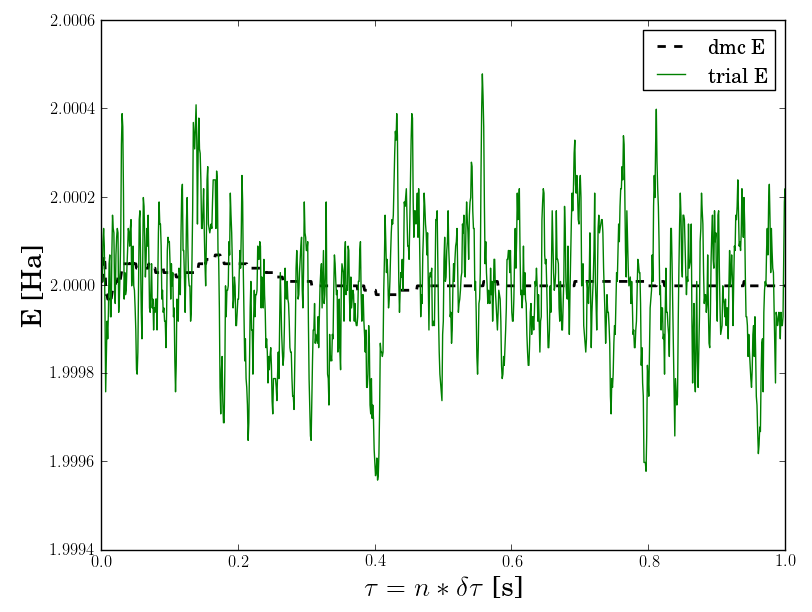
\includegraphics[scale=0.35]{../graphics/DMC_notExactWF.png}
  \end{center}
  \caption{DMC calculation without the exact wave function. The exact result is $E_0=2$. The VMC energy is $2.0042(3)$, whereas the DMC energy is $2.00000(2)$.}
 \end{figure}
\end{frame}







